\documentclass[12pt]{article}

%\usepackage{times} %for Times New Roman, if required
\usepackage[top=1in, bottom=1in, left=1in, right=1in]{geometry} %adjust margins. TODO: hack to fix large top margin
\usepackage{setspace} %allows doublespacing, onehalfspacing, singlespacing
\usepackage{enumitem} %for continuing lists
\usepackage{titling} %for moving the title
\usepackage[normalem]{ulem} %for underlining
\usepackage{graphics}

\begin{document}

\begin{spacing}{.4}
\setlength{\droptitle}{-7em}
\title{CSE 485 Project Initialization}
\author{Connor Alfheim \and Ryan Dougherty \and David Ganey \and Dylan Lusi \and Joseph North \and Ben Roos}
\maketitle
\newpage
\end{spacing}

\begin{spacing}{1.5}

\section{Table of Contents}
\begin{enumerate}
\item Overview
\item Requirements
\item First Semester Plan
\item Conclusion
\end{enumerate}
\newpage

\section{Overview}
\subsection{Introduction}
\emph{NOTE: this is stolen from the Bowman document. We should rewrite this a bit}
\newline \newline
New radio telescopes, including the upcoming Hydrogen Epoch of Reionization Array
(HERA; reionization.org), are the next generation of observational cosmology
telescopes. In many engineering terms these are not the most complicated telescopes
ever built, but they do involve the integration of dozens of independent computer
systems and generate petabytes of highly complex data every year – a situation that is
very new to astronomy projects. Hence, the new telescopes present unique
operational and data analysis challenges, many of which stem from the volume of data
and the complexity of processing the data. Commanding the telescopes and data
processing are much more automatic than with traditional telescopes, but the
operational model and user interfaces for controlling and monitoring the telescopes has
yet to be well-implemented. The top level user interfaces need to be developed so that
users can easily monitor data flow, search meta-data, and initiate pre-defined
processing steps on subsets of the data archive. Partial solutions have been developed
to allow more efficient and routine observing command and analysis, however they still
lack a unified interface -- leaving much of the data hidden. When completed, this
project will be a foundation that enables international teams of astrophysicists and
cosmologists to make important cosmological observations for many years to come.

\subsection{Description}
How does this differ from the introduction?

\subsection{Assumptions}
No significant assumptions will be required for this project. Because the project involves improving an existing system, we are able to know how the system will be used and tailor the performance to those situations.

\newpage

\section{Requirements}
The web system has the following requirements:
\begin{enumerate}
\item The web application should display the current status of the Murchison Widefield Array
	\begin{enumerate}
	\item The application should display the status of the array in a visual format
	\end{enumerate}
\item The application will support user accounts
	\begin{enumerate}
	\item Signing in will be required to act on the website, but not to read it
	\item Users should be able to customize their experience by subscribing to various feeds, modules, etc.
	\item Users can create accounts only with permission from a site admin
	\end{enumerate}
\item The application should support some data processing
	\begin{enumerate}
	\item Data contained in periods during which the MWA had malfunctioning nodes should be flagged
	\end{enumerate}
\item The team should generate an API which allows astronomers with limited knowledge of software development to add, extend, and modify the application functionality.
\end{enumerate}

\subsection{Deliverables}
The team will deliver a functional website running on an EC2 instance. The team will be agile, so as the requirements change, so will the specifics of the delivered website. Accompanying the web platform will be documentation, to maintain extensibility in the future after the conclusion of the project.

\subsection{Use-case diagram}
The use-cases for the website are fairly straightforward. Since the application is primarily a data viewer and status monitor, most use-cases simply involve observing data.
\subsubsection{Figure 1: User with account}
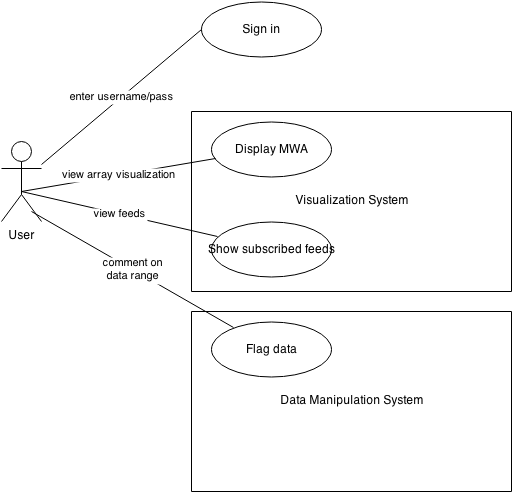
\includegraphics{usecase1} %we can use this to insert .png files in the same directory
\newpage
Users who are not logged in are not permitted to edit the data:
\subsubsection{Figure 2: User without account}
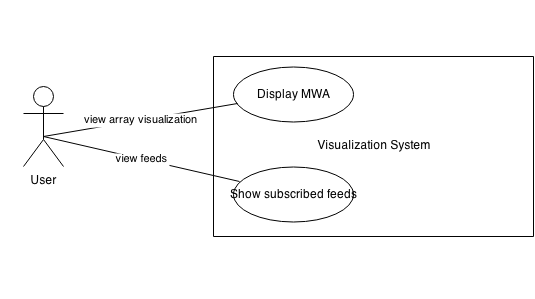
\includegraphics{usecase2}

\subsection{User stories}
\subsubsection{User not signed in}
Users who navigate to the website will see a graphical representation of the Murchison Widefield Array. The visualization will make it clear if any nodes are malfunctioning. Users will be able to see other default data streams on the main page.
\subsubsection{User signed in}
Users who are signed in have additional privileges above standard users. Signed in users have the option to choose which data streams they see through their subscription settings. Additionally, these users can leave comments on data streams to communicate with other users.

\subsection{Non-functional requirements}
The primary goal of the project is \emph{extensibility}. The API developed by the team should allow individuals who are not software developers to modify and add functionality to the website. As a result, scalability and longterm maintainability are significant nonfunctional requirements. Additionally, standard constraints on security and efficiency apply. The website should not be vulnerable to standard exploits (e.g. no passwords stored in plaintext), and should scale appropriately to deliver a pleasant experience to all users.

\newpage

\section{First semester plan}
During the first semester, roles will be assigned to the team. All members should be functional in all areas, but the sponsors and the team agree that some team members will specialize in specific areas (e.g. the database). After dividing roles, the database team will meet with the sponsors to discuss the database schema. Due to the complexity of the database, a small portion of it will be copied to our test instance to be used in testing.
\newline \newline
Once the EC2 instance is up and running with the database, the team will clone the existing code repository to use it as a base. Whether any of the current code remains in the website is a decision the team will make after reviewing the source code itself. The team can then begin to build features. It is likely that the basic login/logout functionality will be built first, followed by the primary visualization dashboards.

\subsection{Initial scope}
The initial goal of the project is to build the framework for the website. Once user functionality is enabled, different view modules will be added. During all this work, the team will make easy extensibility a high priority.

\subsection{Milestones}
\subsubsection{Table 1}
\begin{tabular}{l | l}
Date			&	Goal \\
\hline
10/3/2014		&	Project Initialization form sent to sponsors \\
\hline
10/11/2014		&	Project Initialization form complete \\
\hline
10/20/2014		&	Database copy completed \\
\hline
11/1/2014		&	Begin work \\
\hline
12/6/2014		&	When does class end? \\
\end{tabular}

\end{spacing}
\end{document}

